\chapter{Introduzione ai grafi}

\textbf{Definizione:} Un grafo è una struttura di dati utilizzata per rappresentare le relazioni tra oggetti. Formalmente, un grafo G è una coppia ordinata G = (V, E), dove V rappresenta l'insieme dei nodi (o vertici) e E rappresenta l'insieme degli archi. Gli archi possono essere diretti o non diretti, a seconda che rappresentino una connessione unidirezionale o bidirezionale tra i nodi.

\textbf{Terminologia:}
\begin{itemize}
  \item \textbf{Grado di un nodo:} Il grado di un nodo è il numero di archi che sono connessi ad esso.
  \item \textbf{Percorso:} Un percorso è una sequenza di nodi collegati da archi.
  \item \textbf{Ciclo:} Un ciclo è un percorso che inizia e termina nello stesso nodo.
  \item \textbf{Grafo connesso:} Un grafo connesso è un grafo in cui esiste un percorso tra ogni coppia di nodi.
  \item \textbf{Grafo pesato:} Un grafo pesato è un grafo in cui ogni arco ha un peso o un valore associato.
  \item \textbf{Grafo orientato:} Un grafo orientato è un grafo in cui gli archi hanno una direzione specifica.
\end{itemize}

\textbf{Rappresentazioni:}
\begin{itemize}
  \item \textbf{Matrice di adiacenza:} Una matrice bidimensionale che rappresenta la presenza o l'assenza di un arco tra i nodi.
  \item \textbf{Lista di adiacenza:} Una lista in cui ogni nodo ha un elenco dei suoi nodi adiacenti.
  \item \textbf{Lista degli archi:} Una lista che contiene tutte le coppie di nodi connessi da un arco.
\end{itemize}

La teoria dei grafi offre un ampio spettro di algoritmi e tecniche per lo studio e l'analisi dei grafi. Tra questi, ci sono algoritmi di attraversamento del grafo come la ricerca in profondità (DFS) e la ricerca in ampiezza (BFS), algoritmi per il percorso più breve come l'algoritmo di Dijkstra e algoritmi per la costruzione di alberi di copertura minimi come l'algoritmo di Kruskal.

La teoria dei grafi è una disciplina fondamentale con numerose applicazioni pratiche, che permette di risolvere una vasta gamma di problemi e modellare relazioni complesse tra gli oggetti.
\section{Rappresentazione grafica}
\begin{center}
  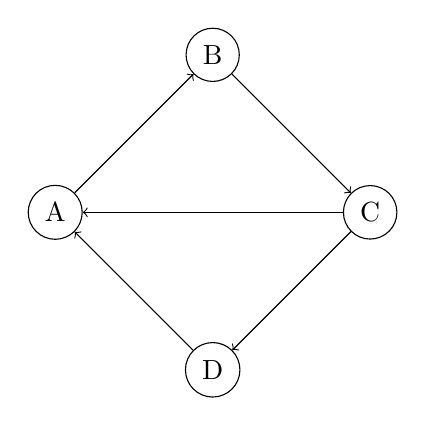
\begin{tikzpicture}
    % Nodi
    \node[draw, circle] (A) at (0,0) {A};
    \node[draw, circle] (B) at (2,2) {B};
    \node[draw, circle] (C) at (4,0) {C};
    \node[draw, circle] (D) at (2,-2) {D};
    
    % Archi
    \draw[->] (A) -- (B);
    \draw[->] (B) -- (C);
    \draw[->] (C) -- (D);
    \draw[->] (C) -- (A);
    \draw[->] (D) -- (A);
  \end{tikzpicture}
\end{center}

\section{Liste di adiacenza}

Le liste di adiacenza sono una delle rappresentazioni più comuni per i grafi. In questa rappresentazione, ogni nodo del grafo è associato a una lista di nodi adiacenti, cioè i nodi che sono direttamente collegati a quel nodo.

Per capire meglio, consideriamo un esempio di un grafo non diretto con 4 nodi (A, B, C, D) e 5 archi (AB, AC, AD, BC, CD). Ecco come potrebbe essere rappresentato utilizzando le liste di adiacenza:

\begin{center}
  \begin{verbatim}
  A: [B, C, D]
  B: [A, C]
  C: [A, B, D]
  D: [A, C]
  \end{verbatim}
\end{center}
Nell'esempio sopra, ogni nodo è seguito da una lista di nodi adiacenti. Ad esempio, il nodo A ha tre nodi adiacenti, che sono B, C e D.

La rappresentazione tramite liste di adiacenza presenta alcuni vantaggi. In primo luogo, è efficiente per i grafi sparsi, cioè quei grafi in cui il numero di archi è molto inferiore al numero massimo possibile di archi. Inoltre, consente di accedere rapidamente ai nodi adiacenti di un dato nodo. Tuttavia, può richiedere più spazio di memoria rispetto ad altre rappresentazioni come le matrici di adiacenza se il grafo ha molti archi.

Le liste di adiacenza sono utilizzate in numerosi algoritmi di grafi, come la ricerca in ampiezza (BFS) e la ricerca in profondità (DFS), poiché consentono un accesso efficiente ai vicini di un nodo.

\section{Matrici di incidenza nodo arco}
Le matrici di incidenza nodo-arco sono una rappresentazione comune per i grafi. In questa rappresentazione, le righe della matrice rappresentano i nodi del grafo e le colonne rappresentano gli archi. Gli elementi della matrice indicano l'incidenza dei nodi sugli archi, cioè se un nodo è collegato o meno a un particolare arco.

Per comprendere meglio, consideriamo un esempio di un grafo diretto con 4 nodi (A, B, C, D) e 5 archi (AB, AC, AD, BC, CD). Ecco come potrebbe essere rappresentato utilizzando una matrice di incidenza nodo-arco:

\begin{center}
\begin{tabular}{c|ccccc}
    & AB & AC & AD & BC & CD \\
\hline
A & -1 & 0 & 0 & 0 & 0 \\
B & 1 & -1 & 0 & 0 & 0 \\
C & 0 & 1 & -1 & 0 & 0 \\
D & 0 & 0 & 1 & -1 & 1 \\
\end{tabular}
\end{center}


Nell'esempio sopra, ogni riga della matrice rappresenta un nodo, mentre ogni colonna rappresenta un arco. Gli elementi della matrice possono assumere i seguenti valori:
\begin{itemize}
  
  \item -1: indica che il nodo è la sorgente dell'arco.
  \item 1: indica che il nodo è la destinazione dell'arco.
  \item 0: indica che il nodo non è collegato all'arco.
\end{itemize}

La rappresentazione tramite matrici di incidenza nodo-arco è particolarmente utile per i grafi con archi diretti e pesati. Questa rappresentazione consente di visualizzare facilmente le connessioni tra i nodi e gli archi del grafo. Tuttavia, rispetto alle liste di adiacenza o alle matrici di adiacenza, le matrici di incidenza richiedono più spazio di memoria e possono essere meno efficienti per alcune operazioni, come la ricerca dei vicini di un nodo.

Le matrici di incidenza nodo-arco sono utilizzate in diversi algoritmi e applicazioni dei grafi, come la risoluzione dei problemi di flusso massimo/minimo e la modellazione di reti di trasporto e comunicazione.


\section{Archi adiacenti e cammini}
Gli archi adiacenti si riferiscono agli archi che condividono un nodo in comune. In altre parole, due archi sono adiacenti se hanno un'estremità comune, che può essere un nodo di partenza o un nodo di arrivo. Ad esempio, se abbiamo un grafo con archi AB, AC e BC, gli archi AB e AC sono adiacenti poiché entrambi hanno il nodo A come estremità iniziale.

I cammini, d'altra parte, sono sequenze ordinate di nodi collegati da archi. Un cammino in un grafo è una serie di nodi in cui ogni coppia consecutiva di nodi è collegata da un arco. Possiamo distinguere diversi tipi di cammini:

\begin{itemize}
  \item Cammino semplice: un cammino in cui nessun nodo appare più di una volta.
  \item Cammino elementare: un cammino in cui nessun arco appare più di una volta.
  \item Cammino ciclo: un cammino in cui il nodo di partenza coincide con il nodo di arrivo.
\end{itemize}

Ad esempio, considera un grafo con i nodi A, B, C e D e gli archi AB, BC e CD. Un possibile cammino in questo grafo potrebbe essere AB-BC-CD, che rappresenta un cammino semplice che connette il nodo A al nodo D attraverso i nodi B e C.

\section{Circuiti hamiltoniani}
Un circuito hamiltoniano in un grafo è un cammino chiuso che attraversa ogni nodo esattamente una volta, ad eccezione del nodo di partenza/arrivo che viene visitato due volte. In altre parole, è un percorso che visita tutti i nodi del grafo una sola volta, ritornando infine al nodo di partenza.

\section{Componenti connesse}
Le componenti connesse sono gruppi di nodi in un grafo che sono collegati tra loro attraverso archi. In altre parole, una componente connessa è un sottoinsieme di nodi di un grafo in cui esiste un percorso tra ogni coppia di nodi all'interno di quella componente.


\subsection{Trovare le componenti connesse}
\begin{lstlisting}
def find_components(graph):
    visited = set()
    components = []

    def dfs(node, component):
        visited.add(node)
        component.append(node)

        for neighbor in graph[node]:
            if neighbor not in visited:
                dfs(neighbor, component)

    for node in graph:
        if node not in visited:
            current_component = []
            dfs(node, current_component)
            components.append(current_component)

    return components

graph = {
    'A': ['B', 'C'],
    'B': ['A', 'C'],
    'C': ['A', 'B'],
    'D': ['E'],
    'E': ['D']
}

components = find_components(graph)
print(components)
\end{lstlisting}


\section{Grafo completo}
Un grafo completo è un tipo particolare di grafo non diretto in cui ogni coppia di nodi è collegata da un arco. In altre parole, in un grafo completo, ogni nodo è connesso direttamente a tutti gli altri nodi del grafo.


\section{Matching}

In teoria dei grafi, un \textit{matching} in un grafo $G = (V, E)$ è un insieme di archi $M \subseteq E$ tale che nessun nodo condivide gli estremi di due archi in $M$.

Formalmente, dato un grafo non diretto $G = (V, E)$, un matching $M$ in $G$ soddisfa le seguenti condizioni:
\begin{enumerate}
    \item Per ogni arco $(u, v) \in M$, nessun arco in $M$ condivide il nodo iniziale $u$ o il nodo finale $v$.
    \item Ogni nodo in $V$ è incidente a al più un arco in $M$.
\end{enumerate}

Un \textit{matching massimale} è un matching che non può essere esteso aggiungendo ulteriori archi senza violare la proprietà di non sovrapposizione. Un \textit{matching perfetto} è un matching in cui tutti i nodi del grafo sono coperti da un arco del matching.

Il matching ha diverse applicazioni, come problemi di assegnazione, progettazione di reti, teoria dei giochi e altro ancora.

\section{Grafi bipartiti}

Un grafo bipartito è un tipo di grafo non diretto in cui i nodi possono essere divisi in due insiemi disgiunti, in modo che ogni arco del grafo colleghi un nodo di un insieme all'altro.

Formalmente, un grafo bipartito $G = (V, E)$ è definito da due insiemi di nodi disgiunti $V1$ e $V2$, dove gli archi del grafo collegano solo i nodi di $V1$ con i nodi di $V2$.

I grafi bipartiti sono rappresentati graficamente come insiemi di punti su due righe parallele, dove gli archi collegano i punti delle due righe.

I grafi bipartiti hanno diverse proprietà interessanti, come la possibilità di essere colorati con solo due colori e l'assenza di cicli di lunghezza dispari.

\subsection{Trovare grafi bipartiti}
\begin{lstlisting}
 
def is_bipartite(graph):
    color = {}
    visited = set()

    def dfs(node, c):
        visited.add(node)
        color[node] = c

        for neighbor in graph[node]:
            if neighbor not in visited:
                if not dfs(neighbor, 1 - c):
                    return False
            elif color[neighbor] == color[node]:
                return False

        return True

    for node in graph:
        if node not in visited:
            if not dfs(node, 0):
                return False

    return True


graph = {
    'A': ['B', 'C'],
    'B': ['A', 'D'],
    'C': ['A', 'D'],
    'D': ['B', 'C']
}

if is_bipartite(graph):
  print("bipartito")
else:
  print("non bipartito")
\end{lstlisting}


\section{Alberi}


Un albero è una struttura dati gerarchica che consiste in un insieme di nodi collegati tra loro in modo specifico. L'albero è composto da una radice, nodi, e archi che connettono i nodi.

I principali termini associati agli alberi sono:

\begin{itemize}
    \item \textbf{Radice}: il nodo di partenza dell'albero.
    \item \textbf{Nodi}: gli elementi dell'albero.
    \item \textbf{Archi}: i collegamenti tra i nodi dell'albero.
    \item \textbf{Figli}: i nodi direttamente collegati a un dato nodo.
    \item \textbf{Genitore}: il nodo da cui un dato nodo è raggiungibile tramite un arco.
    \item \textbf{Foglie}: i nodi che non hanno figli.
    \item \textbf{Livello}: la distanza tra un nodo e la radice.
    \item \textbf{Altezza}: il numero massimo di livelli dell'albero.
\end{itemize}

Gli alberi sono utilizzati in diverse applicazioni, come la rappresentazione delle directory nei sistemi operativi, la gerarchia delle organizzazioni aziendali e la struttura dei dati nelle basi di dati.

\section{Alberi di supporto}
Gli alberi di supporto, noti anche come alberi di copertura o alberi di connessione minima, sono alberi speciali utilizzati in teoria dei grafi. Sono utilizzati per connettere tutti i nodi di un grafo con un numero minimo di archi, garantendo al contempo la connessione tra tutti i nodi.

Formalmente, dato un grafo non diretto ponderato $G = (V, E)$, dove $V$ rappresenta l'insieme dei nodi e $E$ rappresenta l'insieme degli archi, un albero di supporto di $G$ è un sottografo che soddisfa le seguenti proprietà:

\begin{enumerate}
    \item L'albero di supporto contiene tutti i nodi di $G$.
    \item L'albero di supporto è un albero, cioè non contiene cicli.
    \item L'albero di supporto ha il minor peso totale tra tutti gli alberi che soddisfano le prime due proprietà.
\end{enumerate}

Gli alberi di supporto sono utili in diversi contesti, come reti di comunicazione, logistica, progettazione di reti stradali e molto altro ancora.
